\documentclass[landscape,xcolor={table}]{beamer}

\usepackage{amsmath}
\usepackage{graphicx}
\usepackage[english]{babel}
\usetheme{Antibes}
\usepackage{tikz}
\usepackage{multimedia}
\usepackage{textpos}


\usetheme{default}
\usecolortheme{albatross}
\usefonttheme[onlymath]{serif}
\setbeamertemplate{caption}[numbered]
\graphicspath{ {images/} }

\pgfdeclareimage[width=\paperwidth]{mybackground}{images/blue_sun.png}
\pgfdeclareimage[width=0.2\paperwidth]{rocket}{images/launch}

\setbeamertemplate{title page}{

        \begin{picture}(0,0)

            \put(-30,-250){%
                \pgfuseimage{mybackground}
            }

            \put(-168,-100){%
                \begin{minipage}[b][45mm][t]{226mm}
                
                	\centering
               
                  {\usebeamerfont{title}\usebeamercolor{red}\inserttitle \par}
                  
                  \insertauthor
                  
                  \insertinstitute
                  
                  \insertdate
                  
                
                  
                \end{minipage}
            }

            \end{picture}

    }

\title[...]{Hardware and Software Development for \\ MOSES II Flight Operations}
\author[Smart, Remington]{

\includegraphics[width=2cm]{images/moses_logo_with_text} 
\\ Roy Smart \and Jackson Remington}
\institute{Montana State University}
\date{May 1st, 2015 \\ }

\addtobeamertemplate{frametitle}{}{%
\begin{textblock*}{100mm}(.45\textwidth,-1.7cm)

\includegraphics[width=2cm]{images/nasa} \;

\includegraphics[width=2cm]{images/msu}	\;

\includegraphics[width=2cm]{images/ssel}
\end{textblock*}}

	
\begin{document}

	\begin{frame}[plain]
	        \titlepage
	\end{frame}
	
	\begin{frame}
		
		\frametitle{MOSES Scientific Goals}
		
		\begin{columns}[T] % align columns
		\begin{column}{.48\textwidth}

			\begin{itemize}
				\item hey!
			\end{itemize}
			
		\end{column}%
		\hfill%
		\begin{column}{.48\textwidth}
		
			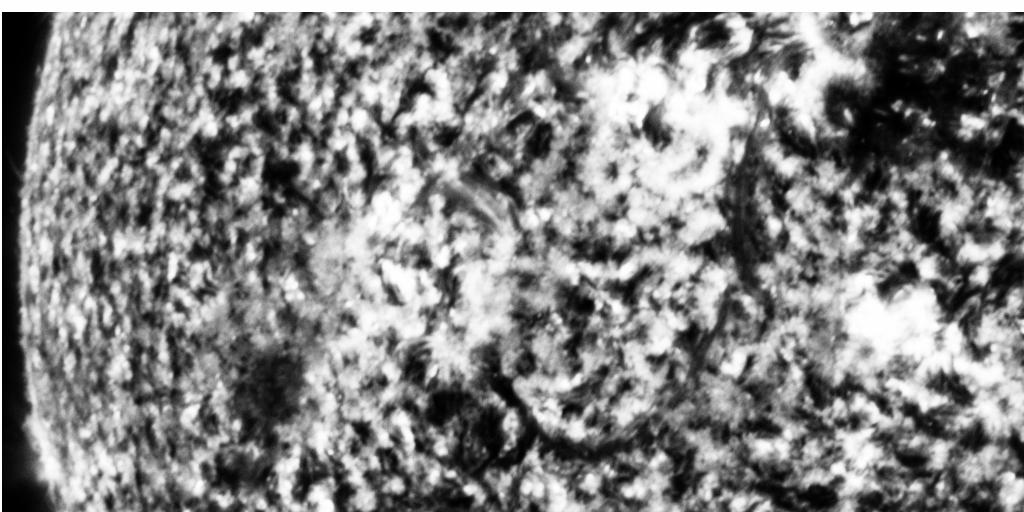
\includegraphics[width=\textwidth]{images/exp2} \\
			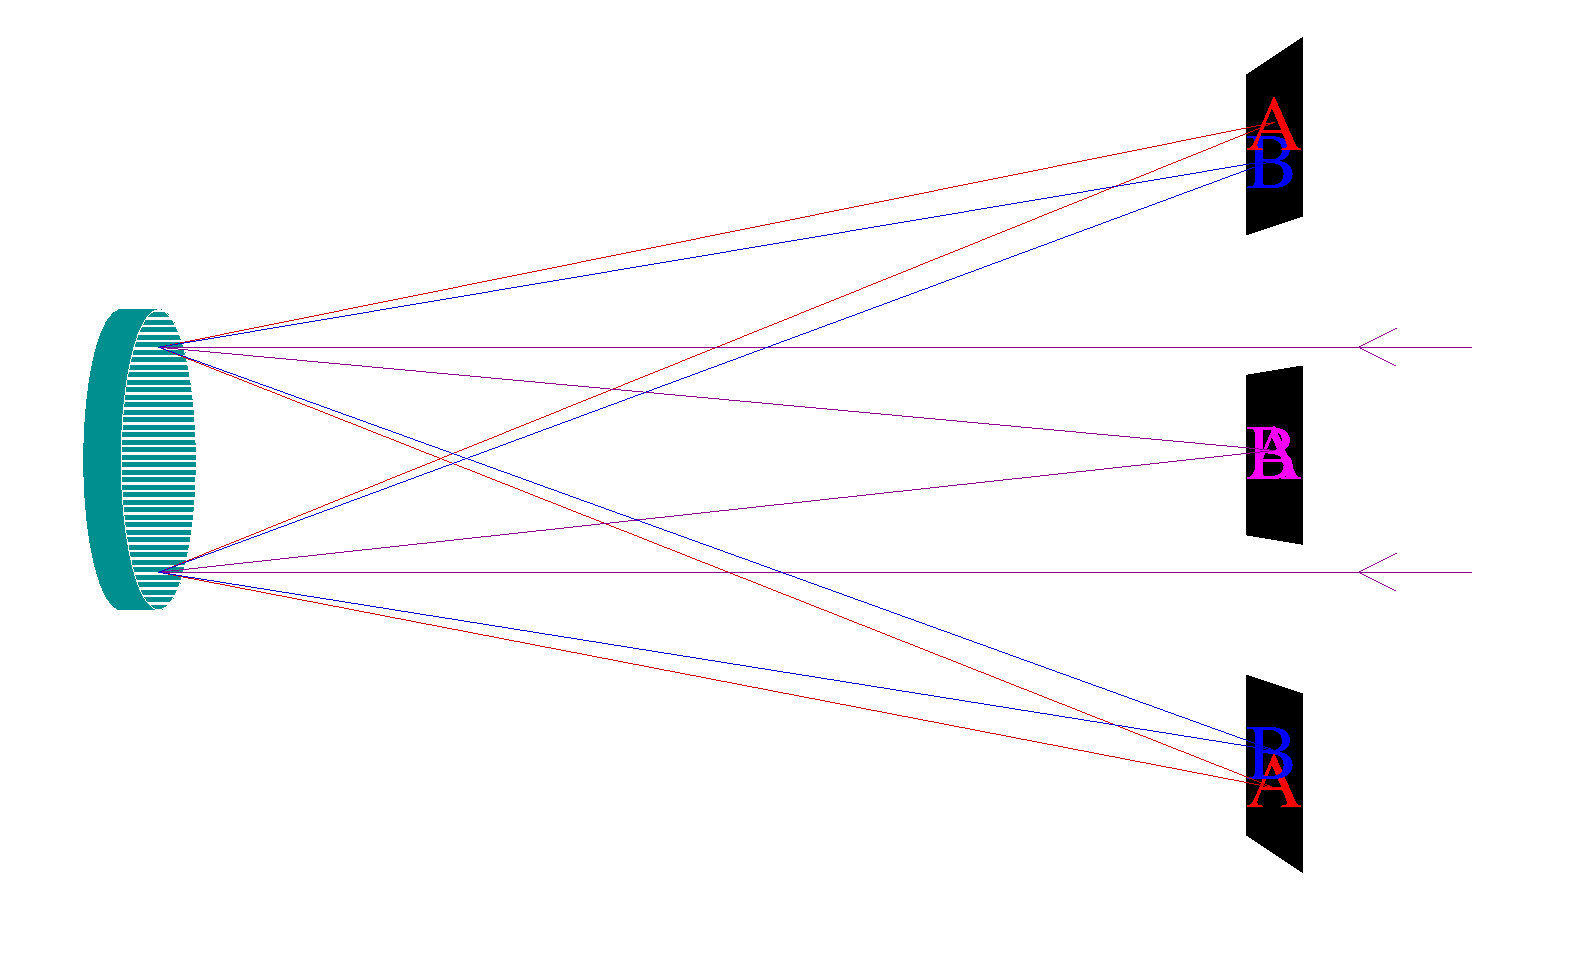
\includegraphics[width=\textwidth]{images/instrument}
		
		\end{column}%
		\end{columns}

	\end{frame}
	
	\begin{frame}
		
		\frametitle{First Launch}
		
		\begin{columns}[T] % align columns
		\begin{column}{.20\textwidth}

			\movie[width=3cm,height=7cm,poster,externalviewer]{\pgfuseimage{rocket}}{images/Launch.mp4}
			
		\end{column}%
		\hfill%
		\begin{column}{.78\textwidth}
		
			\begin{itemize}
				\item hey!
			\end{itemize}
		
		\end{column}%
		\end{columns}
	
	\end{frame}
		
	\begin{frame}
	
		\frametitle{System Requirements}
		
		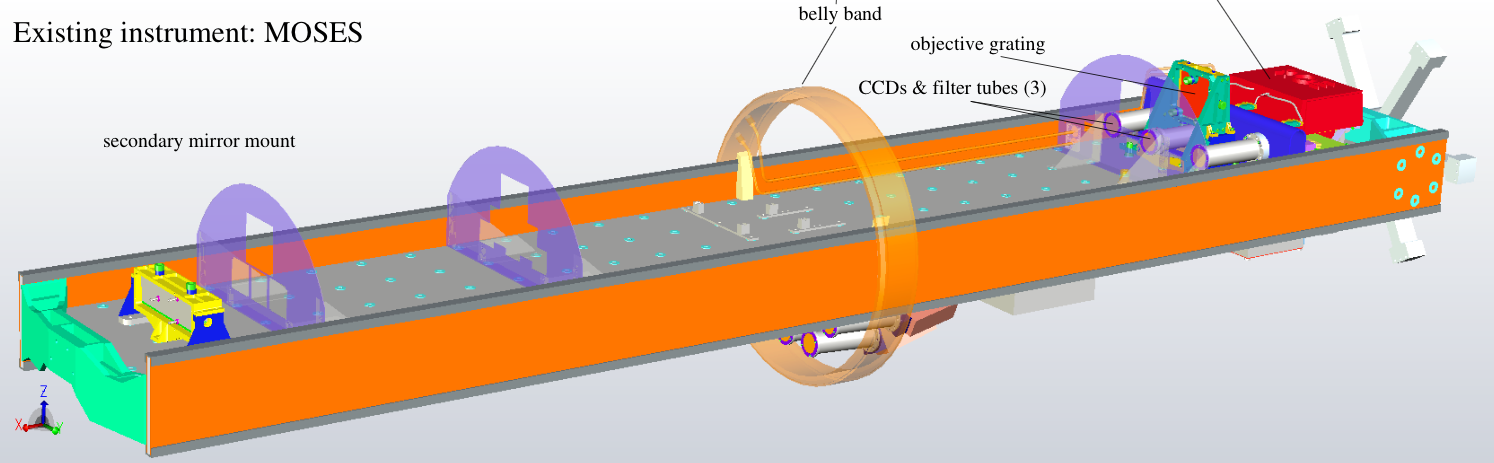
\includegraphics[width=\textwidth]{images/moses}

	\end{frame}
	
	\begin{frame}
		
		\frametitle{Hardware Overview}
		
		\begin{columns}[T] % align columns
		\begin{column}{.68\textwidth}


			
		\end{column}%
		\hfill%
		\begin{column}{.30\textwidth}

			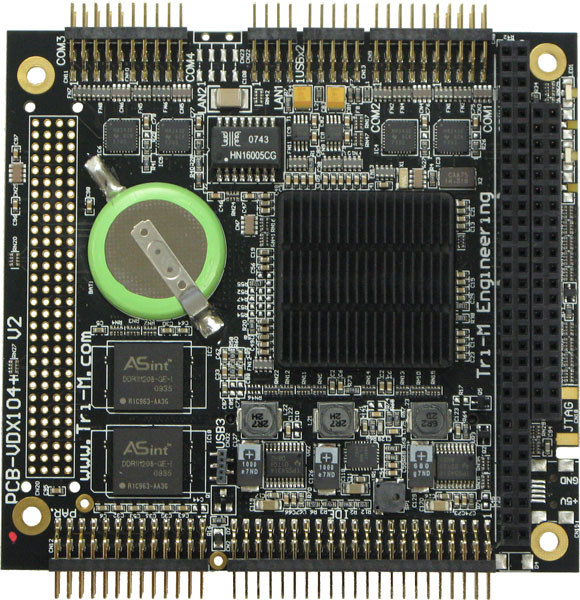
\includegraphics[width=\textwidth]{images/vdx104} \\
			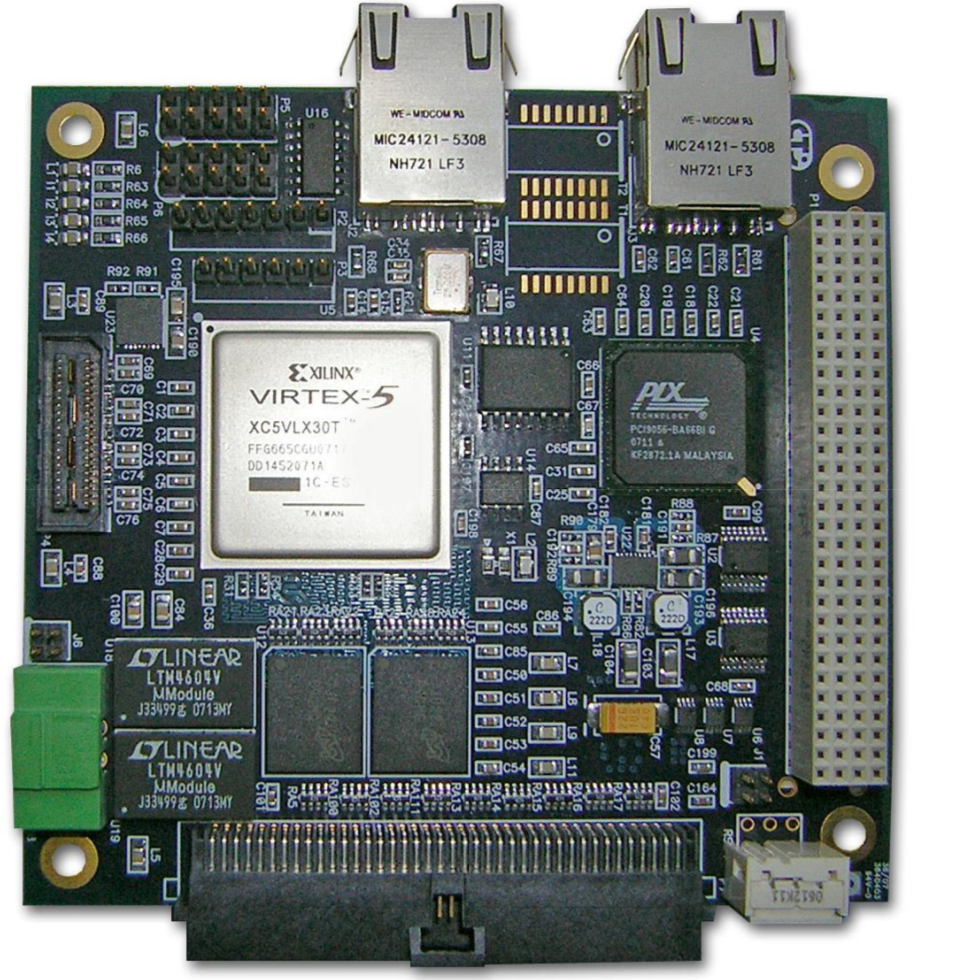
\includegraphics[width=\textwidth]{images/fpga}
					
		\end{column}%
		\end{columns}
			

	\end{frame}
	
	\begin{frame}
		
		\frametitle{Flight Software}
		
		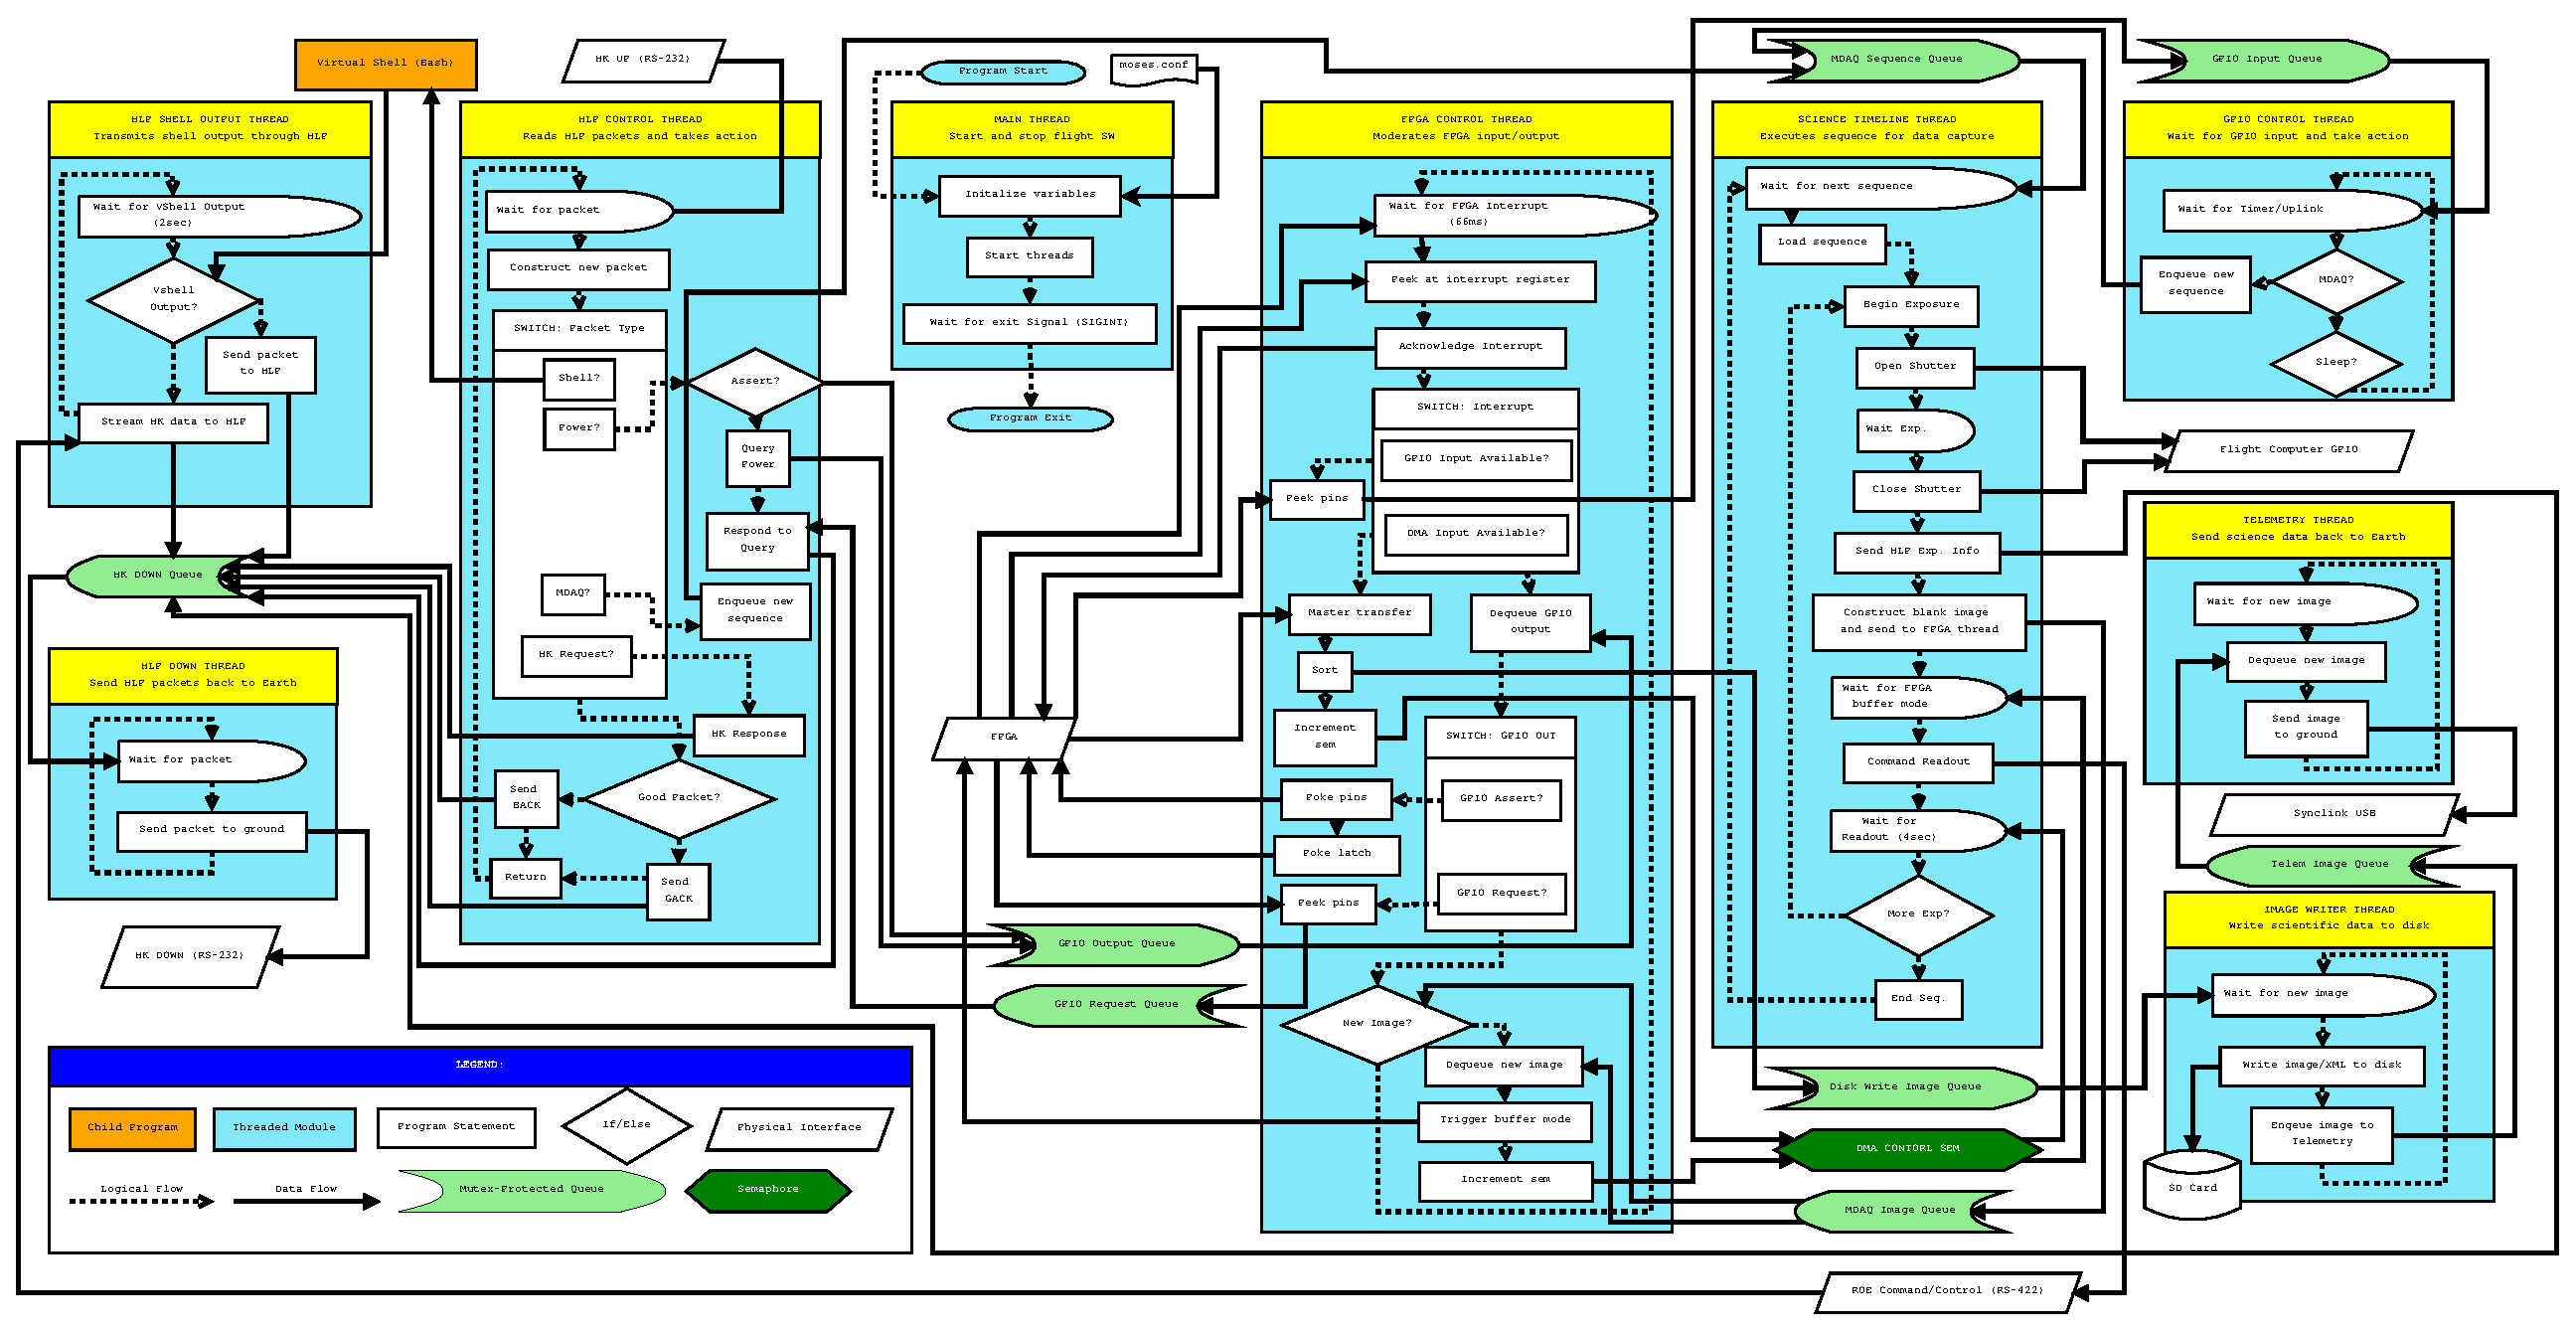
\includegraphics[width=\textwidth]{images/mfsw_block}

	\end{frame}
	
	\begin{frame}
		
		\frametitle{Ground Station Software}
		
		\noindent
		\begin{minipage}[t]{.5\textwidth}
		  
		  \begin{itemize}
		  	\item{Server module}
		  	\item{Client module}
		  	\item{Grounded communication}
		  	\begin{itemize}
		  		\item{Serial console}
		  		\item{Ethernet}
		  	\end{itemize}
		  	\item{In-flight communication}
			\begin{itemize}
		  		\item{Housekeeping Link Protocol (HLP)}
		  		\item{Timers}
		  		\item{High-speed telemetry}
		  	\end{itemize}
		  \end{itemize}
		\end{minipage}
		
		\begin{minipage}[t]{.44\textwidth}
		  
		  \begin{figure}
		  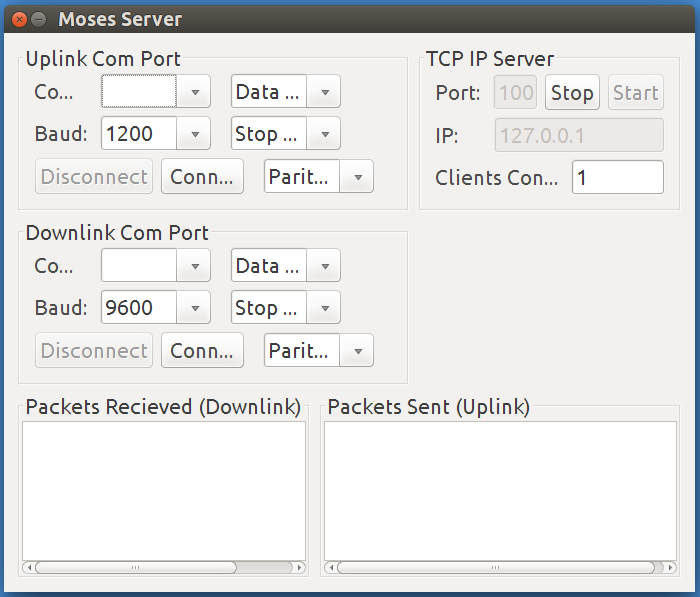
\includegraphics[width=\textwidth]{server_scr}
		  \end{figure}
		  \begin{figure}
 		  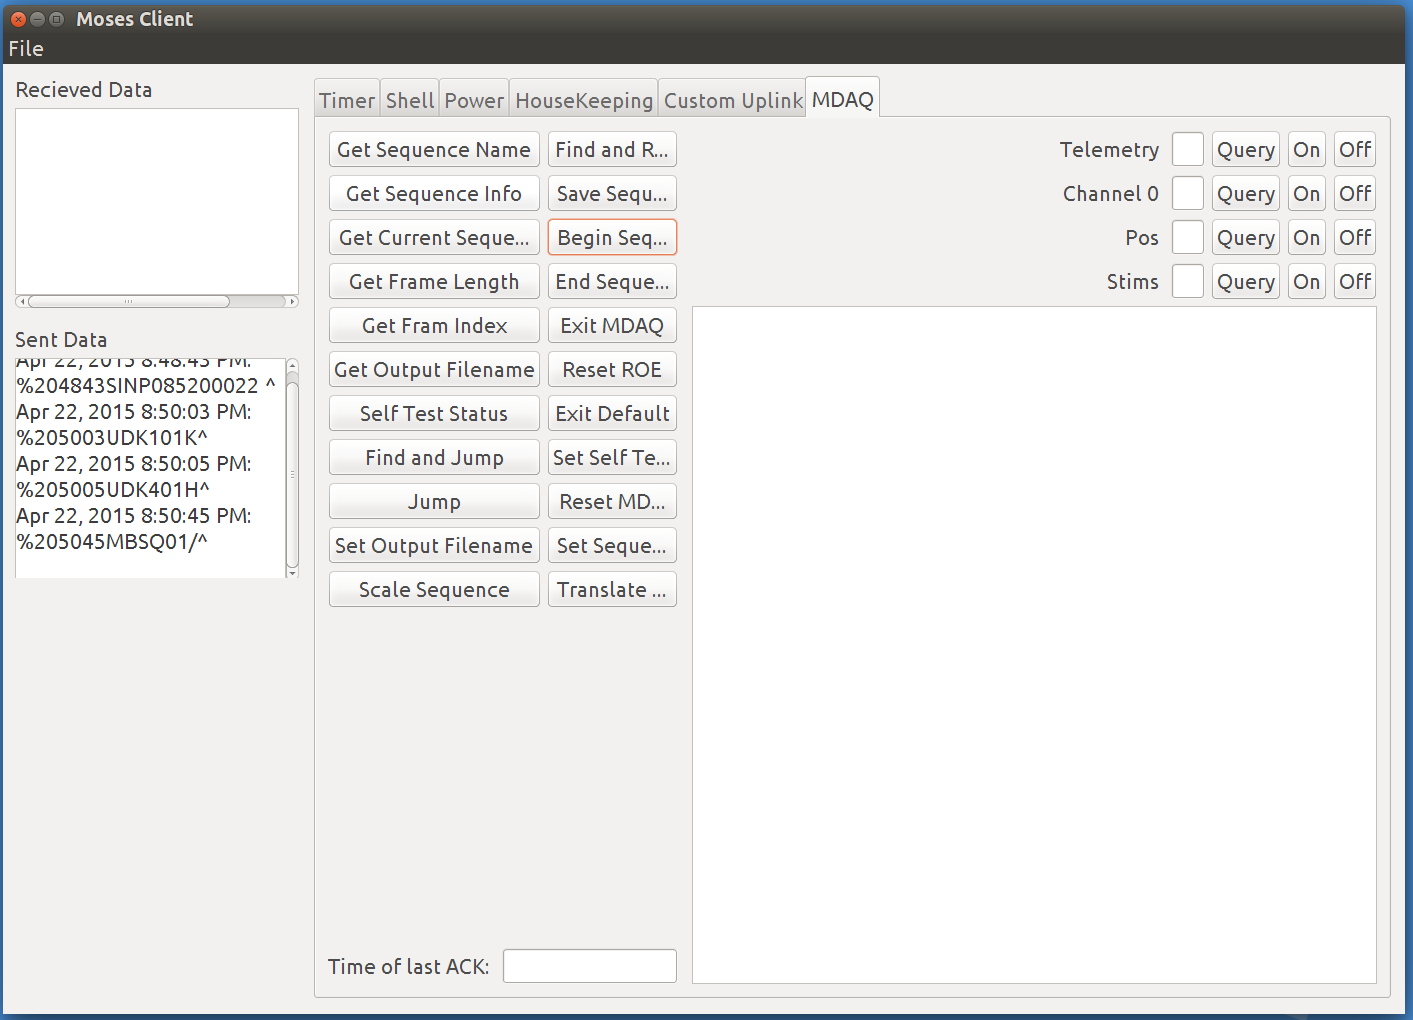
\includegraphics[width=\textwidth]{client_scr}
 		  \end{figure}
		
		\end{minipage}
		
		

	\end{frame}
	
	\begin{frame}
		
		\frametitle{Capturing Data}

	\end{frame}
	
	\begin{frame}
		
		\frametitle{Data Retrieval}

	\end{frame}
	
	\begin{frame}
		
		\frametitle{Next Launch}

	\end{frame}
	
\end{document}








